% \documentclass[varwidth,10pt, border=10pt]{wlscirep}
\documentclass[varwidth, border=10pt, class=wlscirep, 10pt]{standalone}

\RequirePackage{helvet}
\RequirePackage{courier}

% border={10pt 5pt} % left/right bottom/top
% border={10pt 10pt 0pt 10pt} % left right bottom top


\usepackage{subcaption}
\usepackage[
    font=footnotesize,
    labelfont={bf,sf,footnotesize},
    labelsep=period,
    justification=raggedright
]{caption}
\usepackage{graphicx}

\begin{document}

\begin{figure}
    \centering

    \begin{subfigure}[b]{6cm}
        \centering
        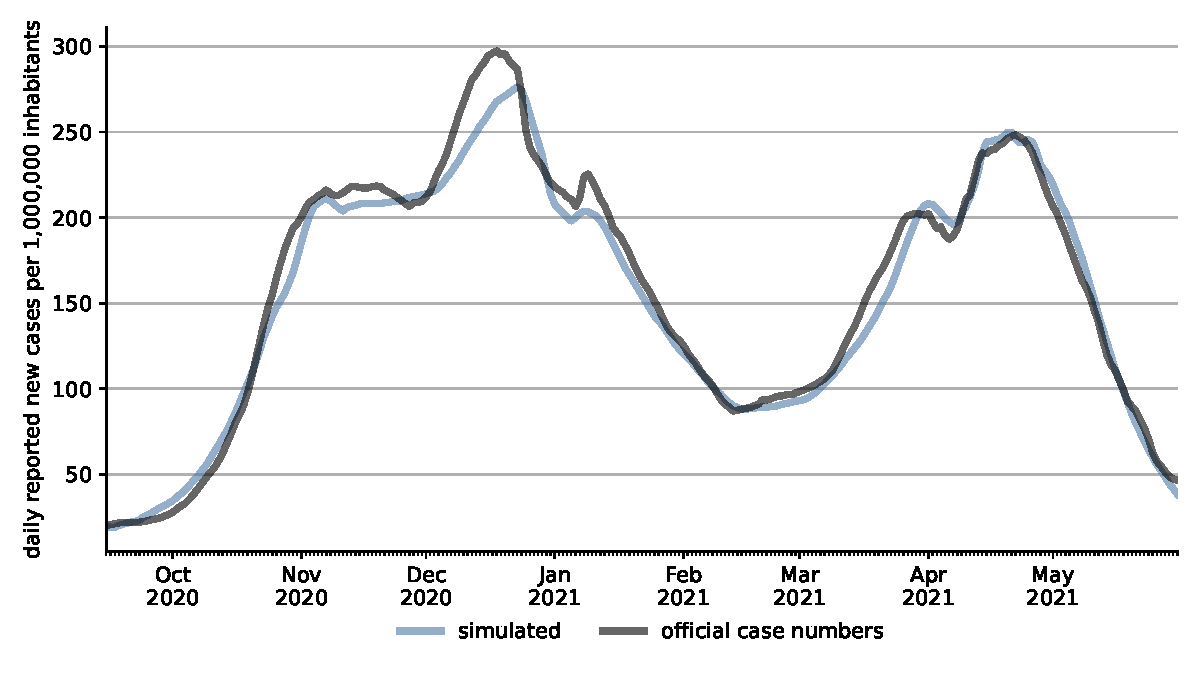
\includegraphics[width=5cm]{../figures/results/figures/scenario_comparisons/combined_fit/full_new_known_case}
        \caption{{Recorded cases: Empirical and simulated}}
        \label{fig:aggregated_fit}
    \end{subfigure}
    \hfill
    \begin{subfigure}[b]{6cm}
        \centering
        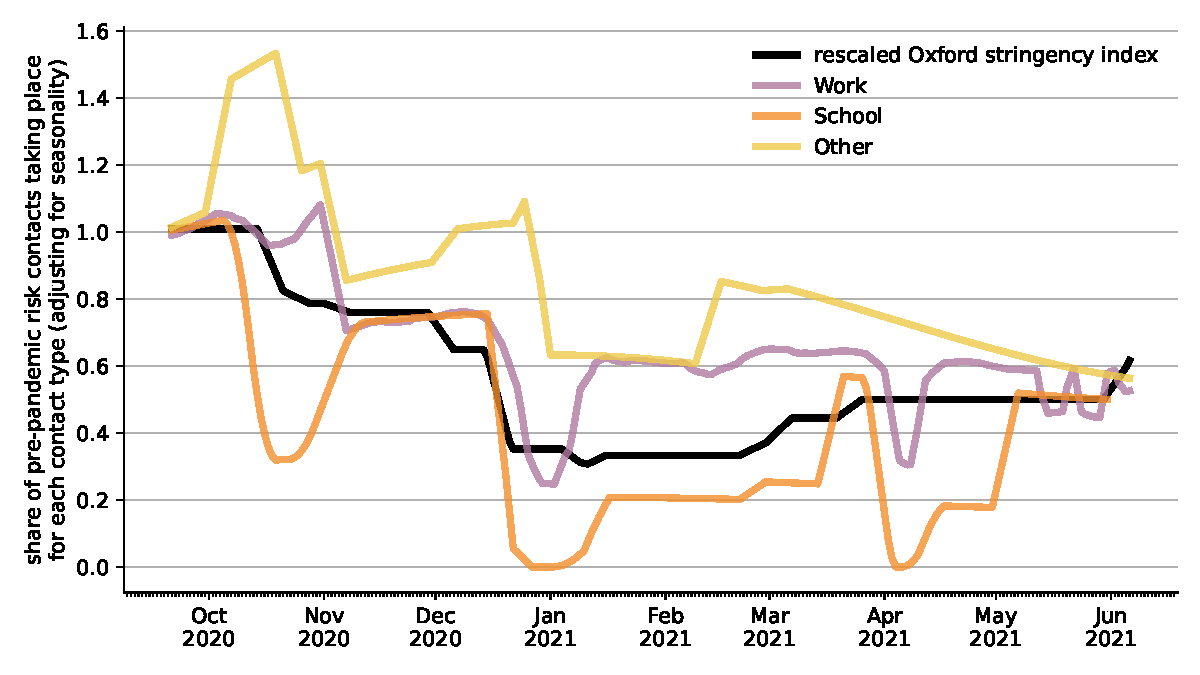
\includegraphics[width=5cm]{../figures/results/figures/data/stringency2_with_seasonality}

        \caption{{Stringency of NPIs and infectious contacts}}
        \label{fig:stringency_infectious_contacts}
    \end{subfigure}
    \vskip3ex
    \begin{subfigure}[b]{6cm}
        \centering

        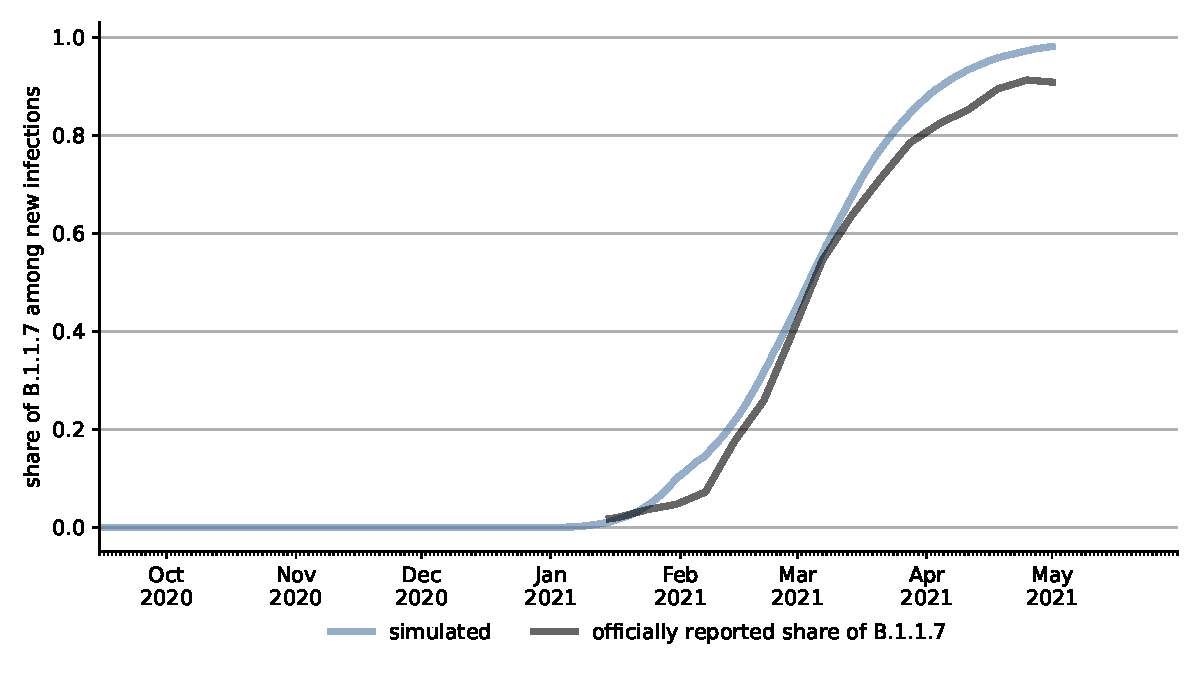
\includegraphics[width=5cm]{../figures/results/figures/scenario_comparisons/combined_fit/full_share_b117}

        \caption{Fraction of B.1.1.7 strain}
        \label{fig:share_b117}
    \end{subfigure}
    \hfill
    \begin{subfigure}[b]{6cm}
        \centering

        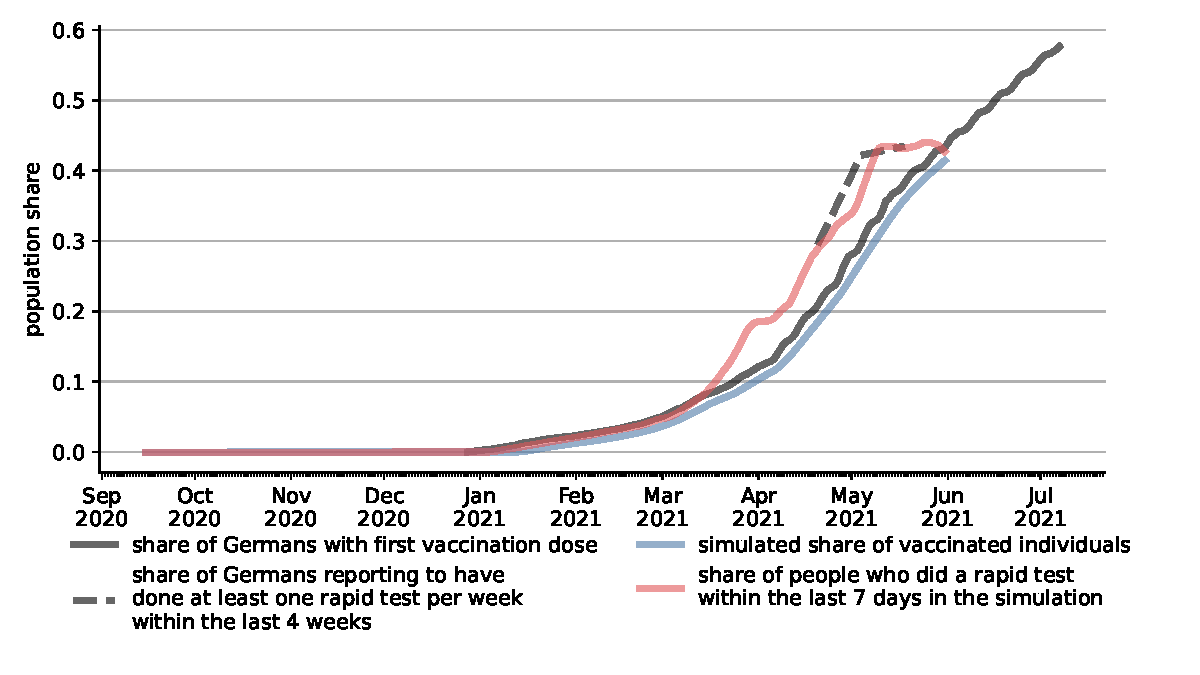
\includegraphics[width=5cm]{../figures/results/figures/scenario_comparisons/combined_fit/full_share_rapid_test_in_last_week_and_vaccinated}

        \caption{{Tests and vaccinations}}
        \label{fig:antigen_tests_vaccinations}
    \end{subfigure}
\end{figure}

\end{document}
